\documentclass[11pt]{article}
%%% Preambuła %%%
\usepackage[T1]{fontenc}
\usepackage[polish]{babel}
\usepackage[utf8]{inputenc}
\usepackage{lmodern}
\usepackage{hyperref}
\usepackage{mathptmx}
\usepackage{float}
\usepackage{graphicx}
\usepackage{xcolor}
\selectlanguage{polish}
\usepackage{titlesec}
\usepackage{listings}


\lstset{
	basicstyle=\ttfamily,
	columns=fullflexible,
	breaklines=true,
	breakatwhitespace=true,
	showstringspaces=false,
	stringstyle = \color{red},
	keywordstyle=\color{blue}
}

\definecolor{backgroundColor}{HTML}{3D3D3D}

%%% Strona tytułowa %%%
\title 
{	
	{
		\textbf{\textsf{\Huge\color{orange}DNS\color{white}ite}} \\ [0.1in]
		\normalfont\sffamily\LARGE\color{white}
		Aplikacja webowa do zarządzania serwerem DNS \\[0.1in]
		Dokumentacja techniczna\\ [1.5in]
		\large 
		Inżynieria Oprogramowania \\
		Wydział Fizyki i Informatyki Stosowanej \\
		Informatyka Stosowana, 3 rok \\
	}
}

\author 
{
	\color{white}\normalfont\sffamily Arkadiusz Kasprzak \and 
	\color{white}\normalfont\sffamily Jarosław Cierpich \and 
	\color{white}\normalfont\sffamily Jakub Kowalski \and 
	\color{white}\normalfont\sffamily Konrad Pasik \and 
	\color{white}\normalfont\sffamily Krystian Molenda
}
\date{}


\definecolor{ao}{rgb}{0.0, 0.0, 1.0}	
\definecolor{forestgreen(web)}{rgb}{0.13, 0.55, 0.13}
\definecolor{darkbrown}{rgb}{0.4, 0.26, 0.13}
\definecolor{darkorange}{rgb}{0.91, 0.41, 0.17}

\titleformat{\section}
  {\normalfont\sffamily\Large\bfseries\color{darkorange}}
  {\thesection}{1em}{}

\titleformat{\subsection}
  {\normalfont\sffamily\large\bfseries\color{darkorange}}
  {\thesubsection}{1em}{}

\titleformat{\subsubsection}
  {\normalfont\sffamily\normalsize\bfseries\color{darkorange}}
  {\thesubsubsection}{1em}{}
	

\begin{document}


%%% Strona tytułowa %%%
\pagecolor{backgroundColor}
\maketitle
\thispagestyle{empty}


\newpage
\clearpage
\pagenumbering{arabic}
\pagecolor{white}

%%% Spis treści %%%
\tableofcontents

\newpage 

\section{Wstęp}
\textbf{DNSite} to aplikacja webowa do zarządzania serwerem DNS. Dostarcza ona użytkownikowi możliwości łatwej i wygodnej edycji danych związanych z serwerem PowerDNS przechowywanych w bazie PostgreSQL.\newline
Niniejsza dokumentacja techniczna została przygotowana dla pierwszego pełnego wydania aplikacji. Zawiera informacje przydatne przy dalszym rozwoju aplikacji.




\section{Budowanie aplikacji}
W celu uruchomienia zbudowania i uruchomienia aplikacji wymagane są:
\begin{itemize}
\item Java w wersji 8
\item Maven
\item Baza danych PostgreSQL 11
\item Aplikacja pgAdmin 4
\end{itemize}
Należy zadbać o to, by przed uruchomieniem aplikacji baza danych była już stworzona - może natomiast nie zawierać tabel.
W celu uruchomienia aplikacji należy pobrać ją z serwisu \textbf{Github} za pomocą polecenia:
\begin{lstlisting}[language=bash]
git clone https://github.com/agh-ki-io/DNSite
\end{lstlisting}
W celach developmentu zaleca się budowanie i uruchamianie aplikacji za pomocą zintegrowanego środowiska programistycznego, np. \textbf{Intellij IDEA}. W tym przypadku należy otworzyć za pomocą tego środowiska projekt, a następnie wykonać na nim operacje \emph{clean} oraz \emph{install} w Mavenie. Po ich zakończeniu należy uruchomić projekt (klasa stanowiąca punkt początkowy to \textbf{DNSiteApplication}). \newline
W wypadku budowania z poziomu konsoli należy natomiast przejść do katalogu \emph{DNSite} i wykonać z jego poziomu polecenie:
\begin{lstlisting}[language=bash]
mvn clean install
\end{lstlisting}
Proces może potrwać kilka minut. Należy zignorować pojawiające się komunikaty (również te oznaczone słowem \emph{error}). Po zakończeniu procesu instalacji sukcesem, w celu uruchomienia aplikacji należy \textbf{z poziomu katalogu DNSite} wykonać polecenie:
\begin{lstlisting}[language=bash]
java -jar target/dnsite-0.0.1-SNAPSHOT.jar
\end{lstlisting}
W przypadku pierwszego uruchomienia pojawi się okno konfiguracji. Proces konfiguracji został szczegółowo opisany w \textbf{Dokumentacji użytkownika} dostępnej dla projektu. Po zakończeniu konfiguracji aplikacja jest dostępna pod adresem: \url{http://localhost:8001/}




\section{Stos technologiczny}
Poniżej przedstawiono stos technologiczny użyty podczas tworzenia aplikacji:
\begin{itemize}
\item \textbf{Baza danych:} PostgreSQL 11
\item \textbf{Backend:}
\begin{itemize}
\item Java 8 (w momencie pisania dokumentacji użycie nowszej wersji nie pozwala na poprawne zbudowanie aplikacji)
\item Framework Spring
\item Spring Boot
\item Spring Security
\item Hibernate
\item JSP
\item log4j
\item snakeyaml
\item gson
\end{itemize}
\item \textbf{Frontend:}
\begin{itemize}
\item React (oraz: react-router, react-table, react-bootstrap)
\item JSP
\item CSS
\end{itemize}
\end{itemize}
Do \textbf{budowania aplikacji} użyty został \emph{Maven}.



\newpage
\section{Warstwa frontend}
Ten rozdział opisuje sposób działania aplikacji po stronie frontendu. Omówione zostaną użyte technologie, organizacja kodu oraz najważniejsze komponenty, w tym komponent tabeli.

\subsection{Użyte technologie}
Pod względem użytych technologii warstwa frontend aplikacji DNSite stanowi hybrydę: główna część aplikacji napisana została z wykorzystaniem biblioteki \textbf{React}, natomiast strony służące m.in. do logowania, rejestracji i przypominania hasła napisane zostały w technologii \textbf{JSP (JavaServer Pages)}. \newline
Hybrydowość warstwy frontend wynika z błędnego początkowego założenia, że cała aplikacja oparta będzie na technologii JSP. Kiedy okazało się, że znacznie wygodniejsze będzie użycie React'a, gotowe były już strony do logowania i rejestracji. Podjęta została decyzja o niewprowadzaniu zmian - wynikło to z obecności innych, ważniejszych dla działania aplikacji, zadań do wykonania.\newline
W nowszej części aplikacji użyte zostały: \emph{React}, \emph{react-router}, \emph{react-bootstrap} oraz \emph{react-table}. Zdecydowaną zaletą React'a jest projektowanie oparte o komponenty. Jest to rozwiązanie, które charakteryzuje prostota i elegancja. Kolejnym ułatwieniem są jasne praktyki dotyczące przepływu danych w aplikacji. Zastosowany wzorzec to jednokierunkowy przepływ danych. Ponadto React jest bardzo wszechstronną oraz popularną biblioteką, posiada zaangażowaną społeczność oraz rozwijany przez nią ekosystem.

\subsection{Organizacja kodu}
Struktura kodu składającego się na warstwę frontend wygląda następująco:
\begin{figure}[H]
\centering
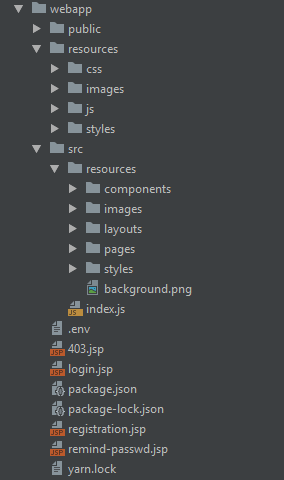
\includegraphics[scale=0.7]{res/front_struktura}
\end{figure}
Część aplikacji wykonana w technologii JSP widoczna jest na dole obrazka - są to pliki:
\begin{itemize}
\item \textbf{403.jsp} - obsługa kodu 403
\item \textbf{login.jsp} - obsługa logowania
\item \textbf{registration.jsp} - obsługa rejestracji nowych użytkowników
\item \textbf{remind-password.jsp} - obsługa panelu przypominania hasła
\end{itemize}
Pliki odpowiadające za \emph{stylowanie} tych stron znajdują się w katalogu \path{webapp\resources}

Część aplikacji zbudowana za pomocą React'a znajduje się natomiast w katalogu \path{webapp\src}. Najważniejsze pliki to:
\begin{itemize}
\item \textbf{App.js} - ogólny komponent, który zbiera wszystkie komponenty
\item \textbf{Footer.js} - komponent odpowiadający za renderowanie stopki aplikacji
\item \textbf{Header.js} - komponent odpowiadający za renderowanie nagłówka aplikacji tj. Tytułu aplikacji
\item \textbf{Navigation.js} - komponent odpowiadający za renderowanie nawigacji aplikacji,
\item \textbf{UserBlock.js} - komponent odpowiadający za renderowanie bloku zawierającego nawigacje do zmiany hasła oraz wylogowania się z aplikacji 
\item \textbf{MainPage.js} - komponent ten wykorzystuje komponenty biblioteki react-router. Dzięki komponentowi Switch w komponencie MainPage zostanie wyrenderowany maksymalnie jeden komponent naraz tj. ten który będzie odpowiadał adresowi URL, natomiast dzięki komponentowi Route możliwe jest określenie jaki komponent ma zostać wyrenderowany w przypadku odwiedzenia odpowiedniego adresu URL, jeżeli podany adres URL nie istnieje, aplikacja komponent Error404, który informuje o błędzie
\item \textbf{ChangePassword.js} - komponent odpowiadający za renderowanie inputów umożliwiających zmianę hasła użytkownika
\item \textbf{Error404.js} - komponent renderuje informacje o błędzie 404
\item \textbf{Home.js} - komponent renderuje informacje o aplikacji oraz o autorach 
\end{itemize}
Pliki \emph{.css} w katalogu \emph{styles} wykorzystywane są do stylowania odpowiadających im komponentów. \newline
W katalogu \emph{images} przechowywane są 2 pliki:
\begin{itemize}
\item \textbf{icon.png} - obraz wykorzystywany jest jako ikona aplikacji w karcie przeglądarki
\item \textbf{background.png} - obraz wykorzystywany jest jako tło fragmentów aplikacji
\end{itemize}



\subsection{Routing}
Do obsługi routingu po stronie przeglądarki wykorzystana została biblioteka \textbf{react-router}. React-router jest bardzo popularną biblioteką, wykorzystywaną często w projektach \emph{SPA (Single-Page Application)}. Dzięki tej bibliotece zapytanie do serwera wykonywane jest wyłącznie raz, na początku działania aplikacji. Po zmianie URL strona nie jest odświeżana, aplikacja przechwytuję zmianę URL i w oparciu o konfigurację Routera wyświetla odpowiedni widok dla danego URL. React-router wykonuje 3 podstawowe funkcje: modyfikuje URL, po wykonaniu modyfikacji ponownie renderuje aplikację, rozpoznaje URL i określa jakie komponenty mają być wyświetlane dla danej lokalizacji. Dzięki bibliotece react-router możemy też wykorzystać interfejs przeglądarki np. cofanie do poprzedniej strony bez odświeżania. 

\subsection{Komponent ReusableTable}
\textbf{TO SIE POJAWI JUTRO}



\section{Warstwa backend}
Ten rozdział opisuje sposób działania aplikacji po stronie backendu. Omówione zostaną rozwiązana stanowiące o przepływie danych w aplikacji, jej bezpieczeństwie, tworzeniu kopii zapasowych danych przechowywanych w bazie, czy tworzących historię operacji na niej.

\subsection{Struktura warstwy backend, rdzeń aplikacji}
Struktura warstwy backend została stworzona w taki sposób, aby być zgodną z ustalonym standardem dla frameworku Spring, czyli dla każdej tabeli w bazie danych, której odwzorowanie tworzymy po stronie backendu tworzona jest następująca struktura pakietów:
\begin{itemize}
\item \textbf{model} - znajduje się tutaj klasa, której pola mapowane są na pola tabeli w bazie danych
\item \textbf{controller} - klasy odpowiadające za przekazywanie requestów między bazą danych oraz frontendem. Wykonują również potrzebne przetworzenia danych. Odpowiadają za dodatkową logikę w związku z DNS (np.: notifiedSerial)\footnote{Duża część \emph{logiki biznesowej} została zaimplementowana po stronie controller, co powinno zostać przeniesione do service. Wynika to z niewystarczającego doświadczenia developerów na początku projektu.}
\item \textbf{service} - odpowiada za logikę dostępu do danych
\item \textbf{repository} - wykorzystuje JPA do dostępu do bazy danych, wykorzystywany przez service
\item \textbf{DTO - Data Transfer Object} - model pozwalający na \emph{obcięcie} danych wysyłanych z rzeczywistego modelu do frontendu. Dodatkowo klasa konwertująca pozwalająca na swobodne przejścia DTO <--> model
\end{itemize}
Poniżej przykład realizacji opisanej struktury dla obsługi \emph{rekordów DNS}:
\begin{figure}[H]
\centering
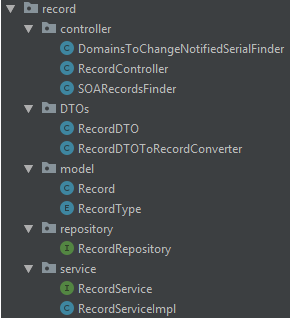
\includegraphics[scale=1]{res/back_struktura}
\end{figure}
oraz przykładowy diagram zależności dla tabeli rekordów:
\begin{figure}[H]
\centering
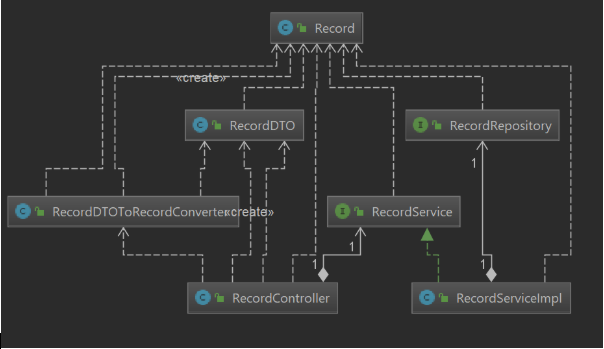
\includegraphics[width=\textwidth]{res/back_diagram_zaleznosci}
\end{figure}
\textbf{Nie wszystkie tabele} wykorzystywane przez PowerDNS zostały zaimplementowane z pełną obsługą. Można je rozpoznać po tym, że wewnątrz ich pakietu znajduje się jedynie pakiet \emph{model}. Są to: tsig\_keys, domain\_meta\_data, cryptokey. 

Oprócz tego w części backendowej aplikacji znajduje się moduł \textbf{utils} w którym znajdują się klasy odpowiedzialne za:
\begin{itemize}
\item Dodatkowe funkcjonalności, np.: BackupPostgresql
\item Adnotacje pozwalające na łatwą walidację danych przekazywanych do modeli, np.: IpAddress oraz IpAddressValidator
\item DTO dla naruszeń walidacji, klasy do zaawansowanego przetwarzania DTO (SOARecordsCreator, DomainIdExtractor)
\item Skonfigurowanie połączenia z bazą danych przy pierwszym uruchomieniu (pakiet hibernate)
\item Wspólną logikę dla notifiedSerial (rekordy SOA w content posiadają również notifiedSerial)
\end{itemize}


\subsection{Logika notifiedSerial}
\textbf{NotifiedSerial} to wartość ustawiana dla \emph{domeny DNS}, pozwalająca na powiadomienie pozostałych serwerów o aktualizacji zawartości domeny. W przypadku, gdy utworzona zostaje nowa domena, do jej pola \emph{notifiedSerial} przypisywana jest następująca wartość typu integer: \emph{YYYYMMDD00} - jest to liczba dziesięciocyfrowa, której pierwsze 8 cyfr przedstawia datę dodania. \newline
Wartość notifiedSerial jest zwiększana w przypadku, gdy któryś rekord typu \textbf{NIE} SOA przypisany do domeny zostanie zmieniony. W przypadku, gdy notfiedSerial jest ustawiony to jest on zwiększany o 1. Jeśli jego wartość nie jest ustawiona, to tworzony jest on na nowo zgodnie z wcześniejszym algorytmem.


\subsection{Bezpieczeństwo i użytkownicy}

W katalogu \textbf{security} znajdują się wszystkie klasy odpowiedzialne za bezpieczeństwo aplikacji. Zostały one napisane głównie przy użyciu \emph{frameworka Spring Security}.

Użytkownicy aplikacji mają przydzielone odpowiednie role:
\begin{itemize}
\item ADMIN - ma dostęp do całej aplikacji, może wykonywać każdą dostępną aplikację, w tym przyznawać innym użytkownikom dostęp do strony. Pierwszy użytkownik aplikacji automatycznie otrzymuje status administratora.
\item USER - jego prawa są ograniczone, nie ma dostępu do głównej części aplikacji. Użytkownik o tym statusie oczekuje na przyznanie dostępu do aplikacji.
\end{itemize} 
Przyznanie użytkownikowi z rolą \emph{USER} dostępu do strony przez administratora zmienia jego rolę na \emph{ADMIN}.

W katalogu \textbf{config} znaleźć można konfigurację odpowiedzialną między innymi za uniemożliwienie użytkownikom korzystania z elementów aplikacji, do których nie mają dostępu. \newline
Linia:
\begin{lstlisting}[language=java]
.antMatchers("/resources/**", "/registration","/remind-passwd").permitAll()
\end{lstlisting}
definiuje miejsca w aplikacji, do których dostęp ma każdy bez względu na swoje uprawnienia. \newline
Kod:
\begin{lstlisting}[language=java]
.loginPage("/login")
\end{lstlisting}
definiuje domyślną stronę logowania. \newline
Linia:
\begin{lstlisting}[language=java]
.exceptionHandling().accessDeniedPage("/403");
\end{lstlisting}
sprawia, że gdy użytkownik próbuje wejść na stronę, do której nie ma dostępu, to otrzymuje on w odpowiedzi stronę z kodem 403. \newline
Hasła są \textbf{hashowane} przy użyciu \textbf{bCryptPasswordEncoder()}.

Warstwa bezpieczeństwa aplikacji zbudowana jest ponadto z następujących klas:
\begin{itemize}
\item \textbf{UserServiceImpl} - pozwala ona na mapowanie obiektów na rekordy w bazie. W funkcji \emph{save} do zapisania hasła używany jest wspomniany wcześniej \emph{enkoder} - hasło nie jest więc przechowywane w postaci czystego tekstu. Klasa ta pozwala również na aktualizację danych w bazie (hasło) czy też przeszukiwanie bazy.
\item \textbf{UserController} - za pomocą tej klasy wystawiane jest API służące późniejszej obsłudze użytkowników po stronie frontendu. Większość funkcji w tej klasie nie wymaga osobnego komentarza - wyjątkiem jest funkcja \emph{registration}, służąca do rejestracji. W tej funkcji początkowo dokonujemy walidacji danych formularza otrzymanych z warstwy frontend. Następnie wykonywane jest sprawdzenie, czy użytkownik jest pierwszym rejestrowanym w aplikacji. Jeśli tak jest, to zostaje on automatycznie zalogowany i przyznana zostaje mu rola ADMIN. W przeciwnym wypadku do wszystkich administratorów wysyłana jest wiadomość e-mail z informacją, że nowy użytkownik oczekuje na przyznanie dostępu do aplikacji. Administratorzy mogą zadecydować o przyjęciu nowego użytkownika.
\item encja \textbf{User} - reprezentuje użytkownika aplikacji w bazie danych. Zawiera następujące atrybuty: \emph{id}, \emph{username}, \emph{password}, \emph{role}, \emph{firstName}, \emph{lastName}, \emph{registrationDate}, \emph{lastLoginDate}, \emph{email}, \emph{isUserAccepted}.
\item \textbf{SecurityServiceImpl} - najważniejszą funkcją w tej klasie jest \emph{autologin}. Jeśli aplikacja wykrywa, że użytkownik jest zalogowany do sesji, to nie jest wymagane ponowne jego logowanie - jest automatycznie przenoszony do aplikacji.
\item \textbf{AdministrationController} - w klasie tej wystawiane jest API służące potwierdzaniu lub odrzucaniu nowych użytkowników.
\item \textbf{EmailServiceImpl} - klasa odpowiadająca za implementację usługi mailowej aplikacji. Korzysta z \emph{MimeMessage}. Istnieją dwa scenariusze użycia tej usługi: 
\begin{itemize}
\item Po rejestracji nowego użytkownika do wszystkich administratorów wysyłana jest wiadomość e-mail z informacją o tym zdarzeniu oraz linkiem aktywacyjnym. 
\item Po wprowadzeniu loginu użytkownika w panelu przypominania hasła, pod adres e-mail powiązany z tym loginem zostaje wysyłane nowe, wygenerowane losowo hasło.
\end{itemize}
\end{itemize}

Warstwa bezpieczeństwa aplikacji korzysta również z modułu \textbf{utils}. Znajdują się w nim narzędzia pomocnicze:
\begin{itemize}
\item Klasa \textbf{PasswordUtils} - zawiera narzędzia takie jak walidacja wprowadzonego hasła zgodnie z założonymi wymaganiami czy też sprawdzenie pakietu danych pobranych podczas zmiany hasła. 
\item Klasa \textbf{PasswordGenerator} - odpowiada za generowanie tymczasowego hasła. Pozwala ona na generowanie hasła dostosowanego do wymagań bezpieczeństwa (wielkie oraz małe litery, cyfry). Przykład użycia klasy PasswordGenerator znajduje się w \emph{PasswordUtils.generateTemporaryPassword()}. Wygenerowane hasło jest wysyłane w wiadomości e-mail do użytkownika, którego login został podany w panelu przypominania hasła. 
\end{itemize}

\subsection{Tworzenie kopii zapasowej danych}
Aplikacja posiada system tworzenia kopii zapasowych danych przechowywanych w bazie (\textbf{backup}). Implementacja tego mechanizmu znajduje się w module \emph{utils}. \newline
Backup jest tworzony przy pomocy klas \emph{ScheduledTasks} oraz \emph{BackupPostgresql}. Pierwsza z wymienionych klas odpowiada za wykonywanie czynności zaraz po uruchomieniu aplikacji (initialDelay = 0) oraz cyklicznie co godzinę pracy (fixedRate=1000*60*60). \newline
Implementacja tworzenia backupu znajduje się w klasie BackupPostgresql. Korzysta ona z pliku konfiguracyjnego aplikacji \emph{dbconfig.yaml} w którym: 
\begin{itemize}
\item \emph{backupLocalization} to ścieżka do katalogu w którym mają być tworzone pliki z kopią zapasową bazy danych.
\item \emph{pg\_dumpLocalization} to ścieżka do narzędzia \textbf{pg\_dump.exe} przy pomocy którego tworzony jest backup bazy danych. 
\end{itemize}
Oba pola muszą być poprawnie podane aby tworzenie kopii zapasowej nie działało. W przypadku nie podania, lub błędnego podania którejś ze ścieżek kopia zapasowa nie będzie tworzona. Do odczytania pliku \emph{dbconfig.yaml} wykorzystywana jest klasa \textbf{DbConfigService}. \newline
Tworzenie kopii zapasowej bazy danych polega na uruchomieniu zewnętrznego procesu z poziomu aplikacji - \path{PostgreSQL\11\bin\pg_dump.exe} wraz z odpowiednimi argumentami wywołania. Jest to oficjalne narzędzie do tworzenia backupu bazy danych w PostgreSQL i  powinno instalować się automatycznie podczas instalacji PostgreSQL. Więcej o pg\_dump.exe można znaleźć pod adresem: \url{https://www.postgresql.org/docs/devel/app-pgdump.html} \newline 
Wszystkie niezbędne informacje do uruchomienia procesu tworzącego kopię zapasową bazy danych znajdują się w pliku \emph{dbconfig.yaml}, który jest odczytywany podczas tworzenia obiektu klasy BackupPostgresql. Pliki z kopią zapasową zapisywane są we wskazanym w \emph{backupLocalization} katalogu w plikach o nazwach tworzonych według formatu \emph{backupddMMyyyy\_HHmmss} - odpowiednio data i godzina wykonania kopii zapasowej - w formacie .sql. Wczytywanie kopii zapasowej z poziomu aplikacji nie jest wspierane. Więcej informacji na temat wczytywania kopii zapasowej można znaleźć pod adresem: \url{http://www.postgresqltutorial.com/postgresql-restore-database/}

\subsection{Tworzenie historii operacji na bazie danych}
Aplikacja zawiera moduł odpowiadający za zbieranie historii operacji na bazie danych. Za każdym razem, gdy wykonywana jest jedna z określonych operacji bazodanowych, do specjalnej tabeli w bazie danych zapisywane są najważniejsze informacje o danej operacji.




\section{Testy}
W katalogu \path{src\test} znajdują się napisane dla aplikacji \textbf{testy jednostkowe}. Testują one komponenty aplikacji napisane w języku Java. Przygotowane zostały za pomocą narzędzie \textbf{JUnit} oraz frameworka \textbf{Mockito}. Testy pokrywają funkcjonalności takie, jak: generowanie haseł czy napisane na potrzeby projektu adnotacje służące do walidacji danych.




\section{Lista możliwych rozszerzeń i poprawek}
Poniżej lista proponowanych przez nas rozszerzeń i poprawek w aplikacji, które ze względu na ograniczony czas trwania projektu nie zostały przez nas wprowadzone:
\begin{itemize}
\item zmiana sposobu działania modułu odpowiedzialnego za historię operacji na bazie danych - powinien on być zbudowany na bazie \textbf{AOP (programowanie aspektowe)}
\item dodanie mechanizmu przywracania bazy danych za pomocą pliku kopii zapasowej
\item przeniesienie logiki biznesowej z klas typu controller do service - dotyczy to m.in. domen i rekordów
\item dodanie brakującej logiki dla niektórych tabel, np. \emph{tsigkeys}
\item zwiększenie restrykcyjności walidacji (np dokładniejsza analiza nazw domen)
\item przeprowadzenie migracji części frontendu wykonanej w technologii JSP do Reacta
\item lepszy podział komponentu \emph{ReusableTable}
\item eliminacja niewykrytych do tej pory błędów w logice tabeli
\item dodanie obsługi mechanizmu \emph{Smart Copy} dla stopki i filtrów w tabeli
\item dodanie możliwości filtrowania zarówno po starej, jak i nowej wartości w wierszu (aktualnie działa tylko dla starej). 
\item wdrożenie obsługi \emph{DNSSEC} do projektu
\item wdrożenie systemu replikacji za pomocą \emph{Slony}
\item wdrożenie frameworka do testów przeprowadzanych po stronie React'a
\item zwiększenie pokrycia kodu testami
\end{itemize}





\end{document}